\documentclass{article}
\usepackage{graphicx}
\usepackage{float}
\usepackage{caption}
\usepackage{subcaption}
\usepackage{booktabs}
\usepackage[margin=1in]{geometry}
\usepackage{hyperref}

\begin{document}

\vspace*{-1.5cm} % pull content toward the top (adjust as needed)
\noindent
\makebox[0pt][l]{%
  \raisebox{-0.4\height}{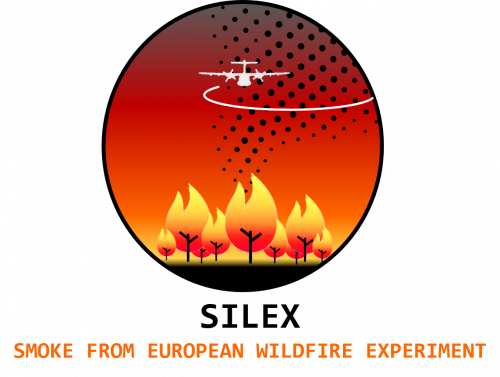
\includegraphics[height=1.4cm]{logo_silex-2-06d25.png}}%
  \hspace{1em}%
  \textbf{\LARGE SILEX Fire Report in France}%
}
\vspace{1cm} % space after title

\section{current status at XX_TIME_REPORT}
Top 10 Fire Events in France by FRP within the last 30min time window processed starting at XX_TIME_REPORT
\begin{table}[H]
\centering
\begin{tabular}{llcc}
\toprule
\textbf{Name} & \textbf{Last Obs} & \textbf{FRP (MW)} & \textbf{Area (km²)} \\
\midrule
XX_TABLE_HERE
\bottomrule
\end{tabular}
\end{table}
\textbf{Number of active fires in France: XX_NUMBER_OF_FIRE } \\
(A fire is considered active in the current version of FET if it has at least one observation within the last 2 days)

\begin{figure}[H]
    \centering
    \begin{subfigure}[b]{0.455\textwidth}
        \centering
        \includegraphics[width=\linewidth]{general_scatterPlot.png} % Replace with actual PNG
    \end{subfigure}
    %\hfill
    \begin{subfigure}[b]{0.535\textwidth}
        \centering
        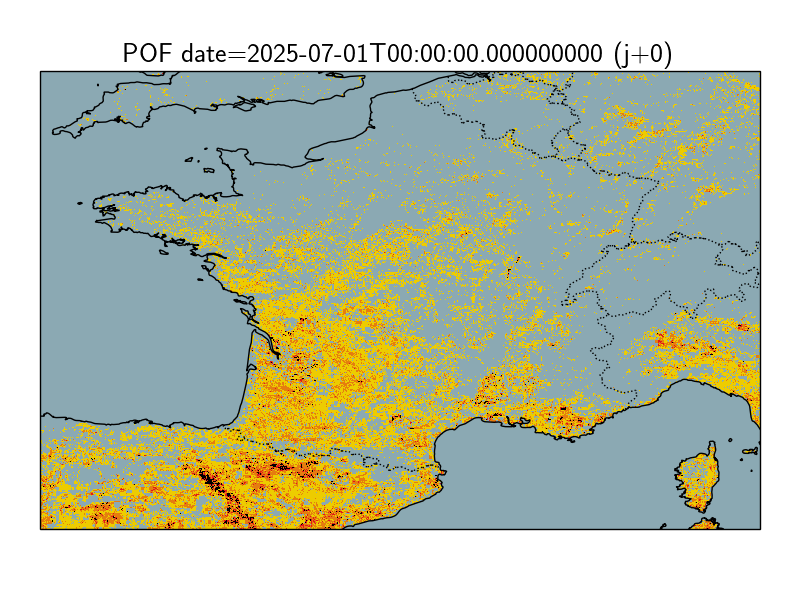
\includegraphics[width=0.85\linewidth]{general_pof_j0.png} % Replace with actual PNG
        \raisebox{4.4mm}{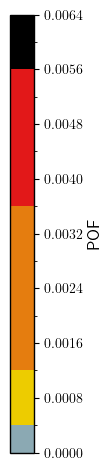
\includegraphics[width=.1275\linewidth]{general_pof_j0_colorbar.png}} % Replace with actual PNG
    \end{subfigure}
\end{figure}

\section{Evolution POF over the next 3 days:}
\begin{figure}[H]
    \centering
    \begin{subfigure}[b]{0.32\textwidth}
        \centering
        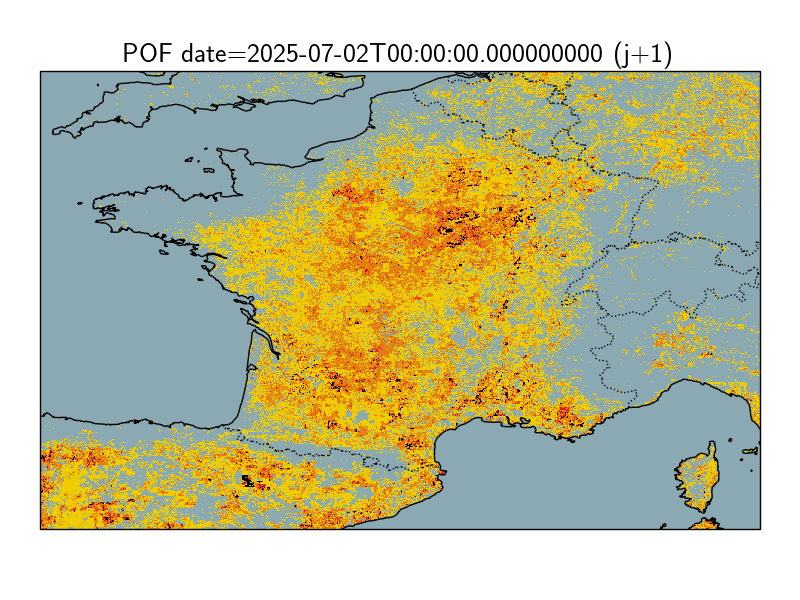
\includegraphics[width=\linewidth]{general_pof_j1.png} % Replace with actual PNG
    \end{subfigure}
    %\hfill
    \begin{subfigure}[b]{0.32\textwidth}
        \centering
        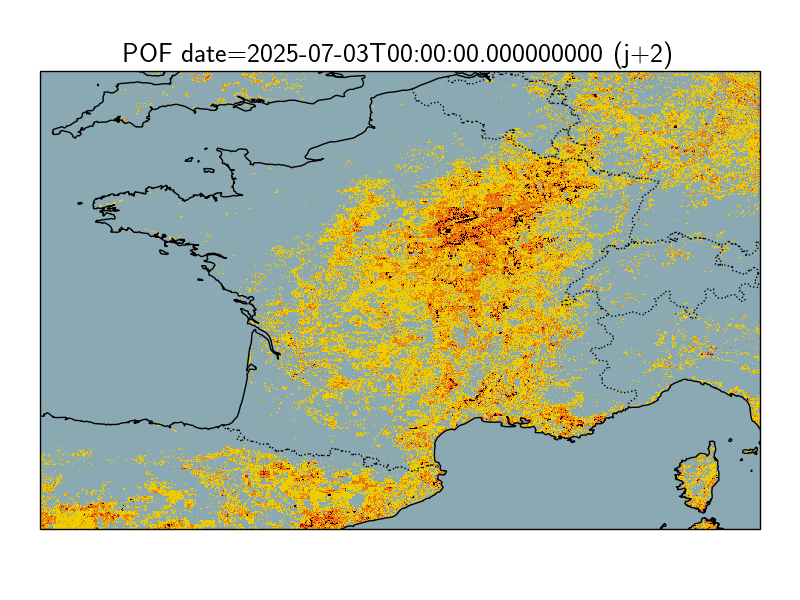
\includegraphics[width=\linewidth]{general_pof_j2.png} % Replace with actual PNG
    \end{subfigure}
    \begin{subfigure}[b]{0.32\textwidth}
        \centering
        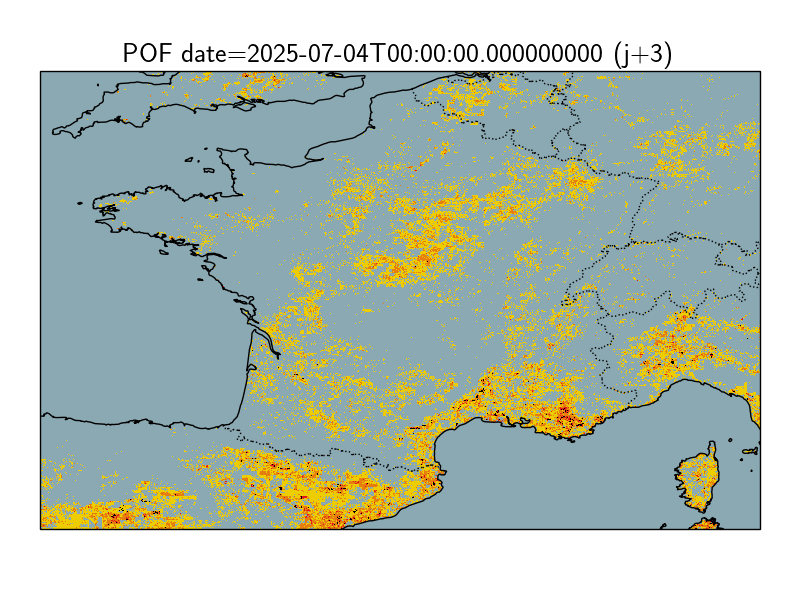
\includegraphics[width=\linewidth]{general_pof_j3.png} % Replace with actual PNG
    \end{subfigure}
\end{figure}



\end{document}
